\chapter{Digital Flow}
\label{chapter:digital-flow}

The goal of this chapter is to present an evolution process that decreases digital elastica energy and can be used in practice. In particular, an application in image segmentation is presented at the end of the chapter. We begin this chapter by pointing a link between the sum of squared disk areas and squared curvature.

\section{Symmetric disks and squared curvature}

Let $\mathcal{C}$ a oriented curve in the plane. We center disks $B_i$ and $B_o$ of radius $R+\epsilon$ with centers aligned with the normal direction of the curve at some point $p \in \mathcal{C}$. Moreover, the distance from disks center to $p$ equals to $R$.

\begin{figure}[h!]\label{fig:r-separated-disks}
\center
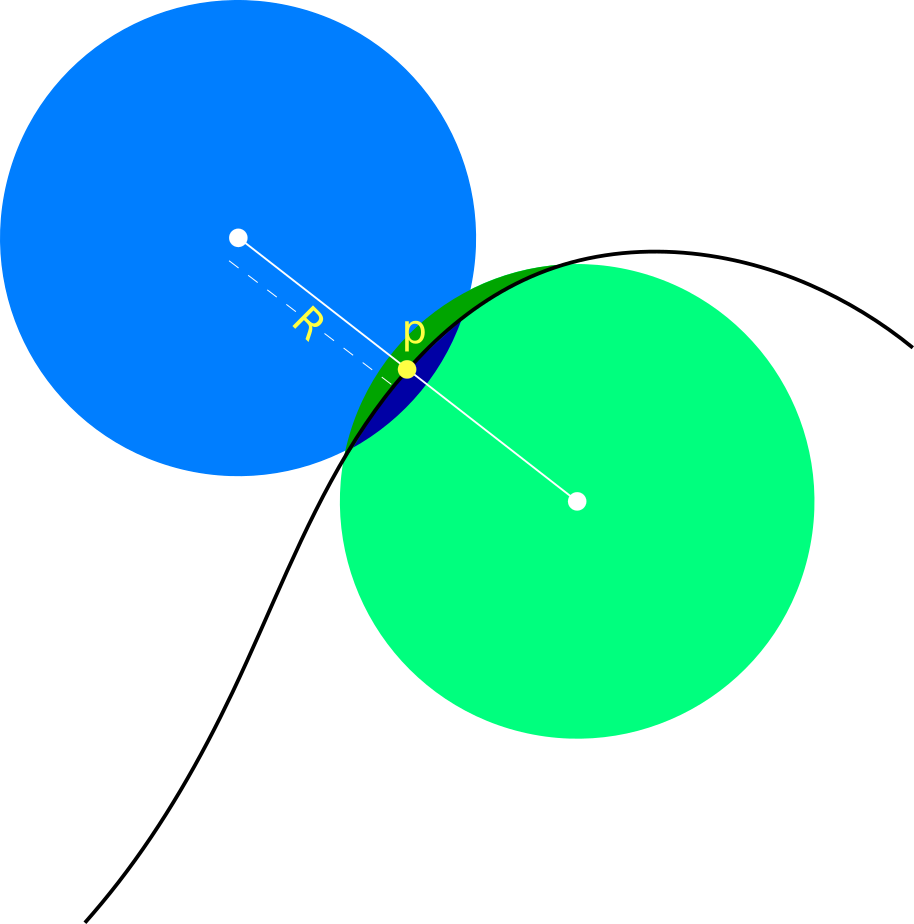
\includegraphics[scale=0.35]{figures/chapter5/max-energy/r-separated-disks.png}
\caption{disks of radius $R+\epsilon$ distant $R$ units from $p\in \mathcal{C}$ in the normal direction.}
\end{figure}

Let $\theta_o (\theta_i)$ to denote the intersection of $B_o(B_i)$ with the inner(outer) region of the curve. We define the function $g:\mathcal{R} \times \mathcal{C}\rightarrow \mathbb{R}$ as

\begin{align*}
	g(\epsilon,p) &= \Big(\; \pi (R+\epsilon)^2 - \Theta_o(p) \; \Big)^2 + \Big(\pi (R+\epsilon)^2 - \Theta_i(p) \;\Big)^2\\
		 &= g_o(\epsilon,p) + g_i(\epsilon,p)
\end{align*}

\begin{claim}{R-separated disks curvature}\label{claim:r-separated-disks}
 Let $\mathcal{C} \in \mathbb{R}^2$ be a curve such that for a point $p \in \mathcal{C}$ its curvature equals to $\kappa$. For sufficiently small values of $\epsilon$ and $\kappa$, we can approximate $g$ by


%No power
%- sqrt(2)*E^(3/2)*R^(5/2)*k^2 + \frac{71}{420}*sqrt(2)*E^(7/2)*R^{-3/2} + 2*pi*E^2 + 4*pi*E*R + 2*pi*R^2 - 14/15*sqrt(2)*E^(5/2)/sqrt(R) - 8/3*sqrt(2)*E^(3/2)*sqrt(R)

%g(\epsilon,p) \approx & -\sqrt{2}\epsilon^{3/2}R^{5/2}\kappa^2 + 2\pi\epsilon^2 + 4\pi\epsilon R + 2\pi R^2 \\
%&- \frac{14}{15}\sqrt{2}\epsilon^{5/2}R^{-1/2} - \frac{8}{3}\sqrt{2}\epsilon^{3/2}\sqrt{R} - \frac{71}{420}\sqrt{2}\epsilon^{7/2}R^{-3/2} 


%Power2
%-2*sqrt(2)*pi*E^(3/2)*R^(9/2)*k^2 + 2*pi^2*R^4 + 8*pi^2*E*R^3 - 16/3*sqrt(2)*pi*E^(3/2)*R^(5/2) + 12*pi^2*E^2*R^2 - 188/15*sqrt(2)*pi*E^(5/2)*R^(3/2) + 8/9*(9*pi^2 + 8)*E^3*R - 611/70*sqrt(2)*pi*E^(7/2)*sqrt(R)   + 2/45*(45*pi^2 + 112)*E^4 



\begin{align*}
g(\epsilon,p) \approx & -2\sqrt{2}\pi\epsilon^{3/2}R^{9/2}\kappa^{2} + 2\pi^2R^4 + 8\pi^2\epsilon R^3 - \frac{16}{3}\sqrt{2}\pi \epsilon^{3/2}R^{5/2} + 12\pi^2 \epsilon^2R^2 \\
& - \frac{188}{15}\sqrt{2}\pi \epsilon^{5/2}R^{3/2} + \frac{8}{9}\big(9\pi^2 + 8\big)\epsilon^3 R - \frac{611}{70}\sqrt{2}\pi \epsilon^{7/2}\sqrt{R} + \frac{2}{45}\big( 45\pi^2 + 112\big)\epsilon^4
\end{align*} 
\end{claim}


\begin{proof} For every point $p$ in $C$, consider its Frenet frame formed by the tangent vector at $p$, $T(p)$ and the normal vector at $p$, $N(p)$. We assume the origin of the frame is at point $p$. Let $x$ be a variable in the axis defined by $T(p)$. Expanding $C(x)$ around the origin we obtain

\begin{align*}
	C(x) &= C(0) + \frac{dC}{dx}x + \frac{1}{2}\frac{d^2C}{dx^2}x^2 + O(x^3) \\
	&= \frac{\kappa}{2}x^2 + O(x^3).
\end{align*}

In other words, the second order approximation for the curve $C$ in the Frenet frame is the parabola $f(x) =  \kappa/2x^2$ passing at the origin. We are going to use this parabola to estimate $g_o$ and $g_i$.

We proceed by computing the intersection area $\theta_o$.


\begin{figure}[h!]\label{fig:parabola-approx-ex}
\center
	\subfloat[\label{}]{%
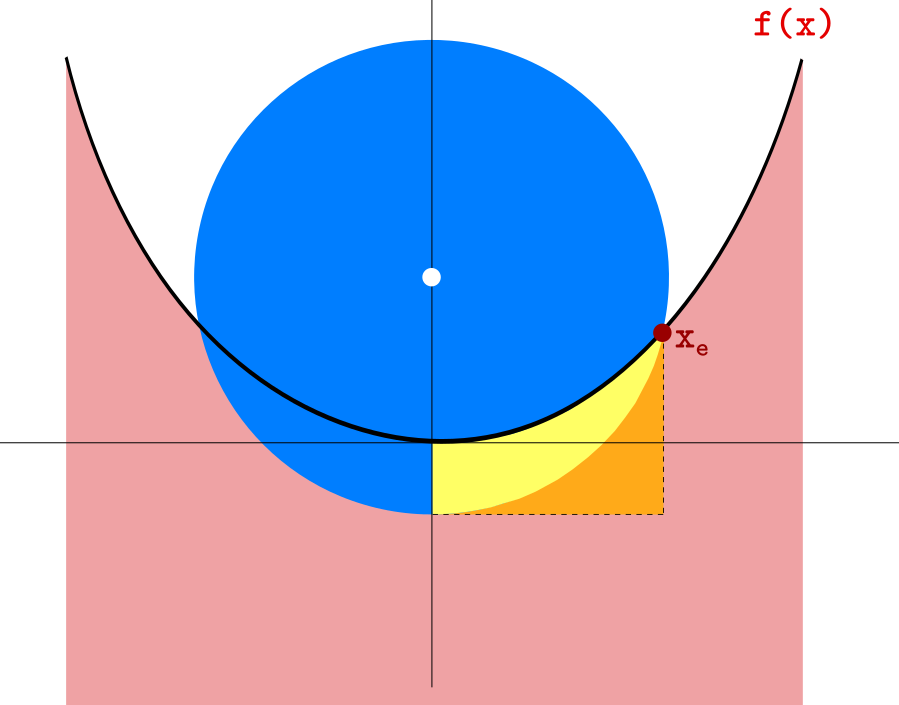
\includegraphics[scale=0.35]{figures/chapter5/max-energy/parabola-approx-1.png}
	}\hspace{20pt}%
	\subfloat[\label{}]{%
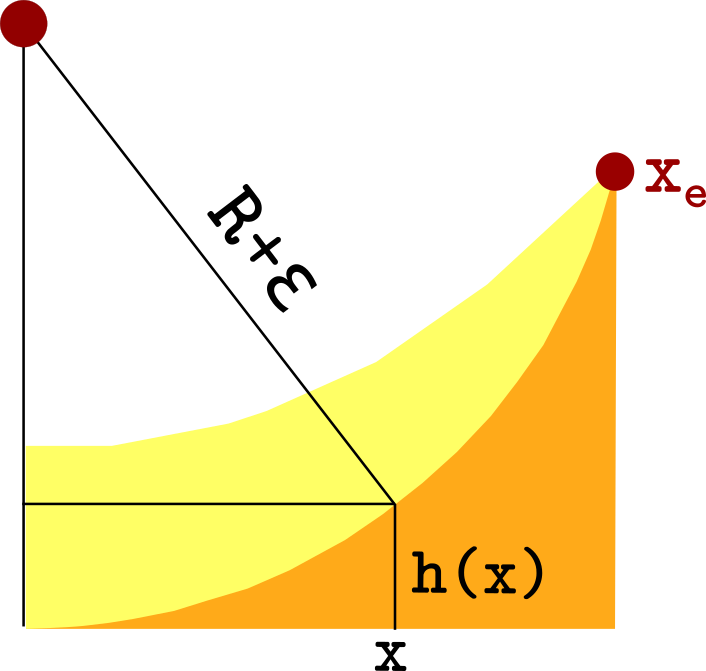
\includegraphics[scale=0.35]{figures/chapter5/max-energy/parabola-approx-2.png}
	}
\caption{The yellow area corresponds to $\theta_o$ and it equals the area under the parabola from $x=0$ until $x=x_o$ minus the orange area $h(x)$.}
\end{figure}

\begin{align*}
	h(x) &= R+\epsilon - \sqrt{ (R+\epsilon)^2 - x^2}\\
	\theta_o &= 2\int_0^{x_o}{f(x) + \epsilon - h(x)}\\
\end{align*}

To compute the intersection point $x_o$ of the parabola with the disc, we use again pythagoras' theorem.

\begin{align*}
	(R+\epsilon)^2 &= (R-\frac{\kappa}{2}x_o^2)^2 + x_o^2\\
	0 &= \frac{\kappa^2}{4}x_o^4 + (1-R\kappa)x_o^2 + R^2 - (R+\epsilon)^2
\end{align*}

By setting $z_o=x_o^2$

\begin{align*}
\Delta_o &= (1-R\kappa)^2 + \kappa^2(2R\epsilon + \epsilon^2)\\
z_o &= \frac{2}{\kappa^2}(R\kappa-1 + \sqrt{\Delta_o})\\
x_o &= \frac{\sqrt{2}}{\kappa}\sqrt{R\kappa-1+\sqrt{\Delta_o}}
\end{align*}

We proceed similarly for the inner disk.


\begin{figure}[h!]\label{fig:parabola-approx-in}
\center
	\subfloat[\label{}]{%
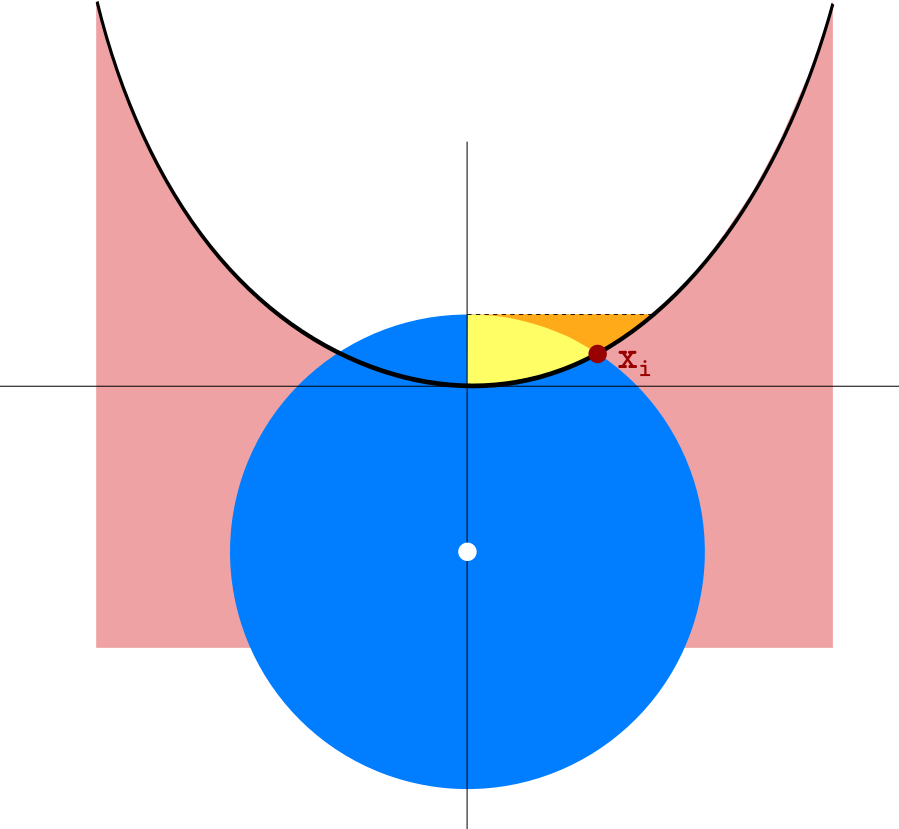
\includegraphics[scale=0.35]{figures/chapter5/max-energy/parabola-approx-3.png}
	}\hspace{15pt}%
	\subfloat[\label{}]{%
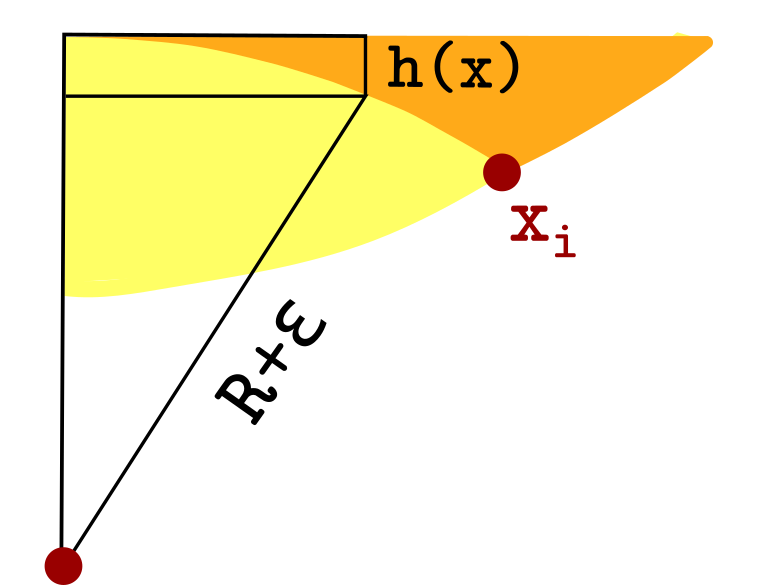
\includegraphics[scale=0.35]{figures/chapter5/max-energy/parabola-approx-4.png}
	}
\caption{The yellow area corresponds to $\theta_i$ and it equals the area between the parabola and the disc from $x=0$ until $x=x_i$.}
\end{figure}

\begin{align*}
	\theta_i &= 2\int_{0}^{x_i}{\epsilon - f(x) - h(x)}	\end{align*}

The intersection point $x_i$ between the parabola and the inner disk is given by
	
\begin{align*}
	(R+\epsilon)^2 &= (R+\frac{\kappa}{2}x_o^2)^2 + x_i^2\\
	0 &= \frac{\kappa^2}{4}x_i^4 + (1+R\kappa)x_i^2 + R^2 - (R+\epsilon)^2	\\
\Delta_i &= (1+R\kappa)^2 + \kappa^2(2R\epsilon + \epsilon^2)\\
x_i &= \frac{\sqrt{2}}{\kappa}\sqrt{-R\kappa-1+\sqrt{\Delta_i}}.
\end{align*}

The claimed approximation is obtained by expanding $g$ with its  4th order Taylor series around $\kappa=0,\epsilon=0$.
\end{proof}

\section{Experimental validation}

We check if $g_{\epsilon,p}$ can be used as squared curvature estimator. It seems that in order to achieve higher precision we need a large radius and a small $\epsilon$.



\section{Curve evolution process}

Given a closed oriented curve $\mathcal{C}$, we define the optimization region $O$ as the band of size $\epsilon /2$ around $\mathcal{C}$. For a given radius $R$, we define the ring $\mathcal{R}$ as

\begin{align*}
	x \in \mathcal{R} \implies \min_{p \in \mathcal{C}} d(x,p) = R.
\end{align*}

The ring is composed of two connected components, denoted here as $C_{inn}$ and $C_{out}$ accordingly with the curve orientation.


\begin{figure}[h!]\label{fig:integral}
\center
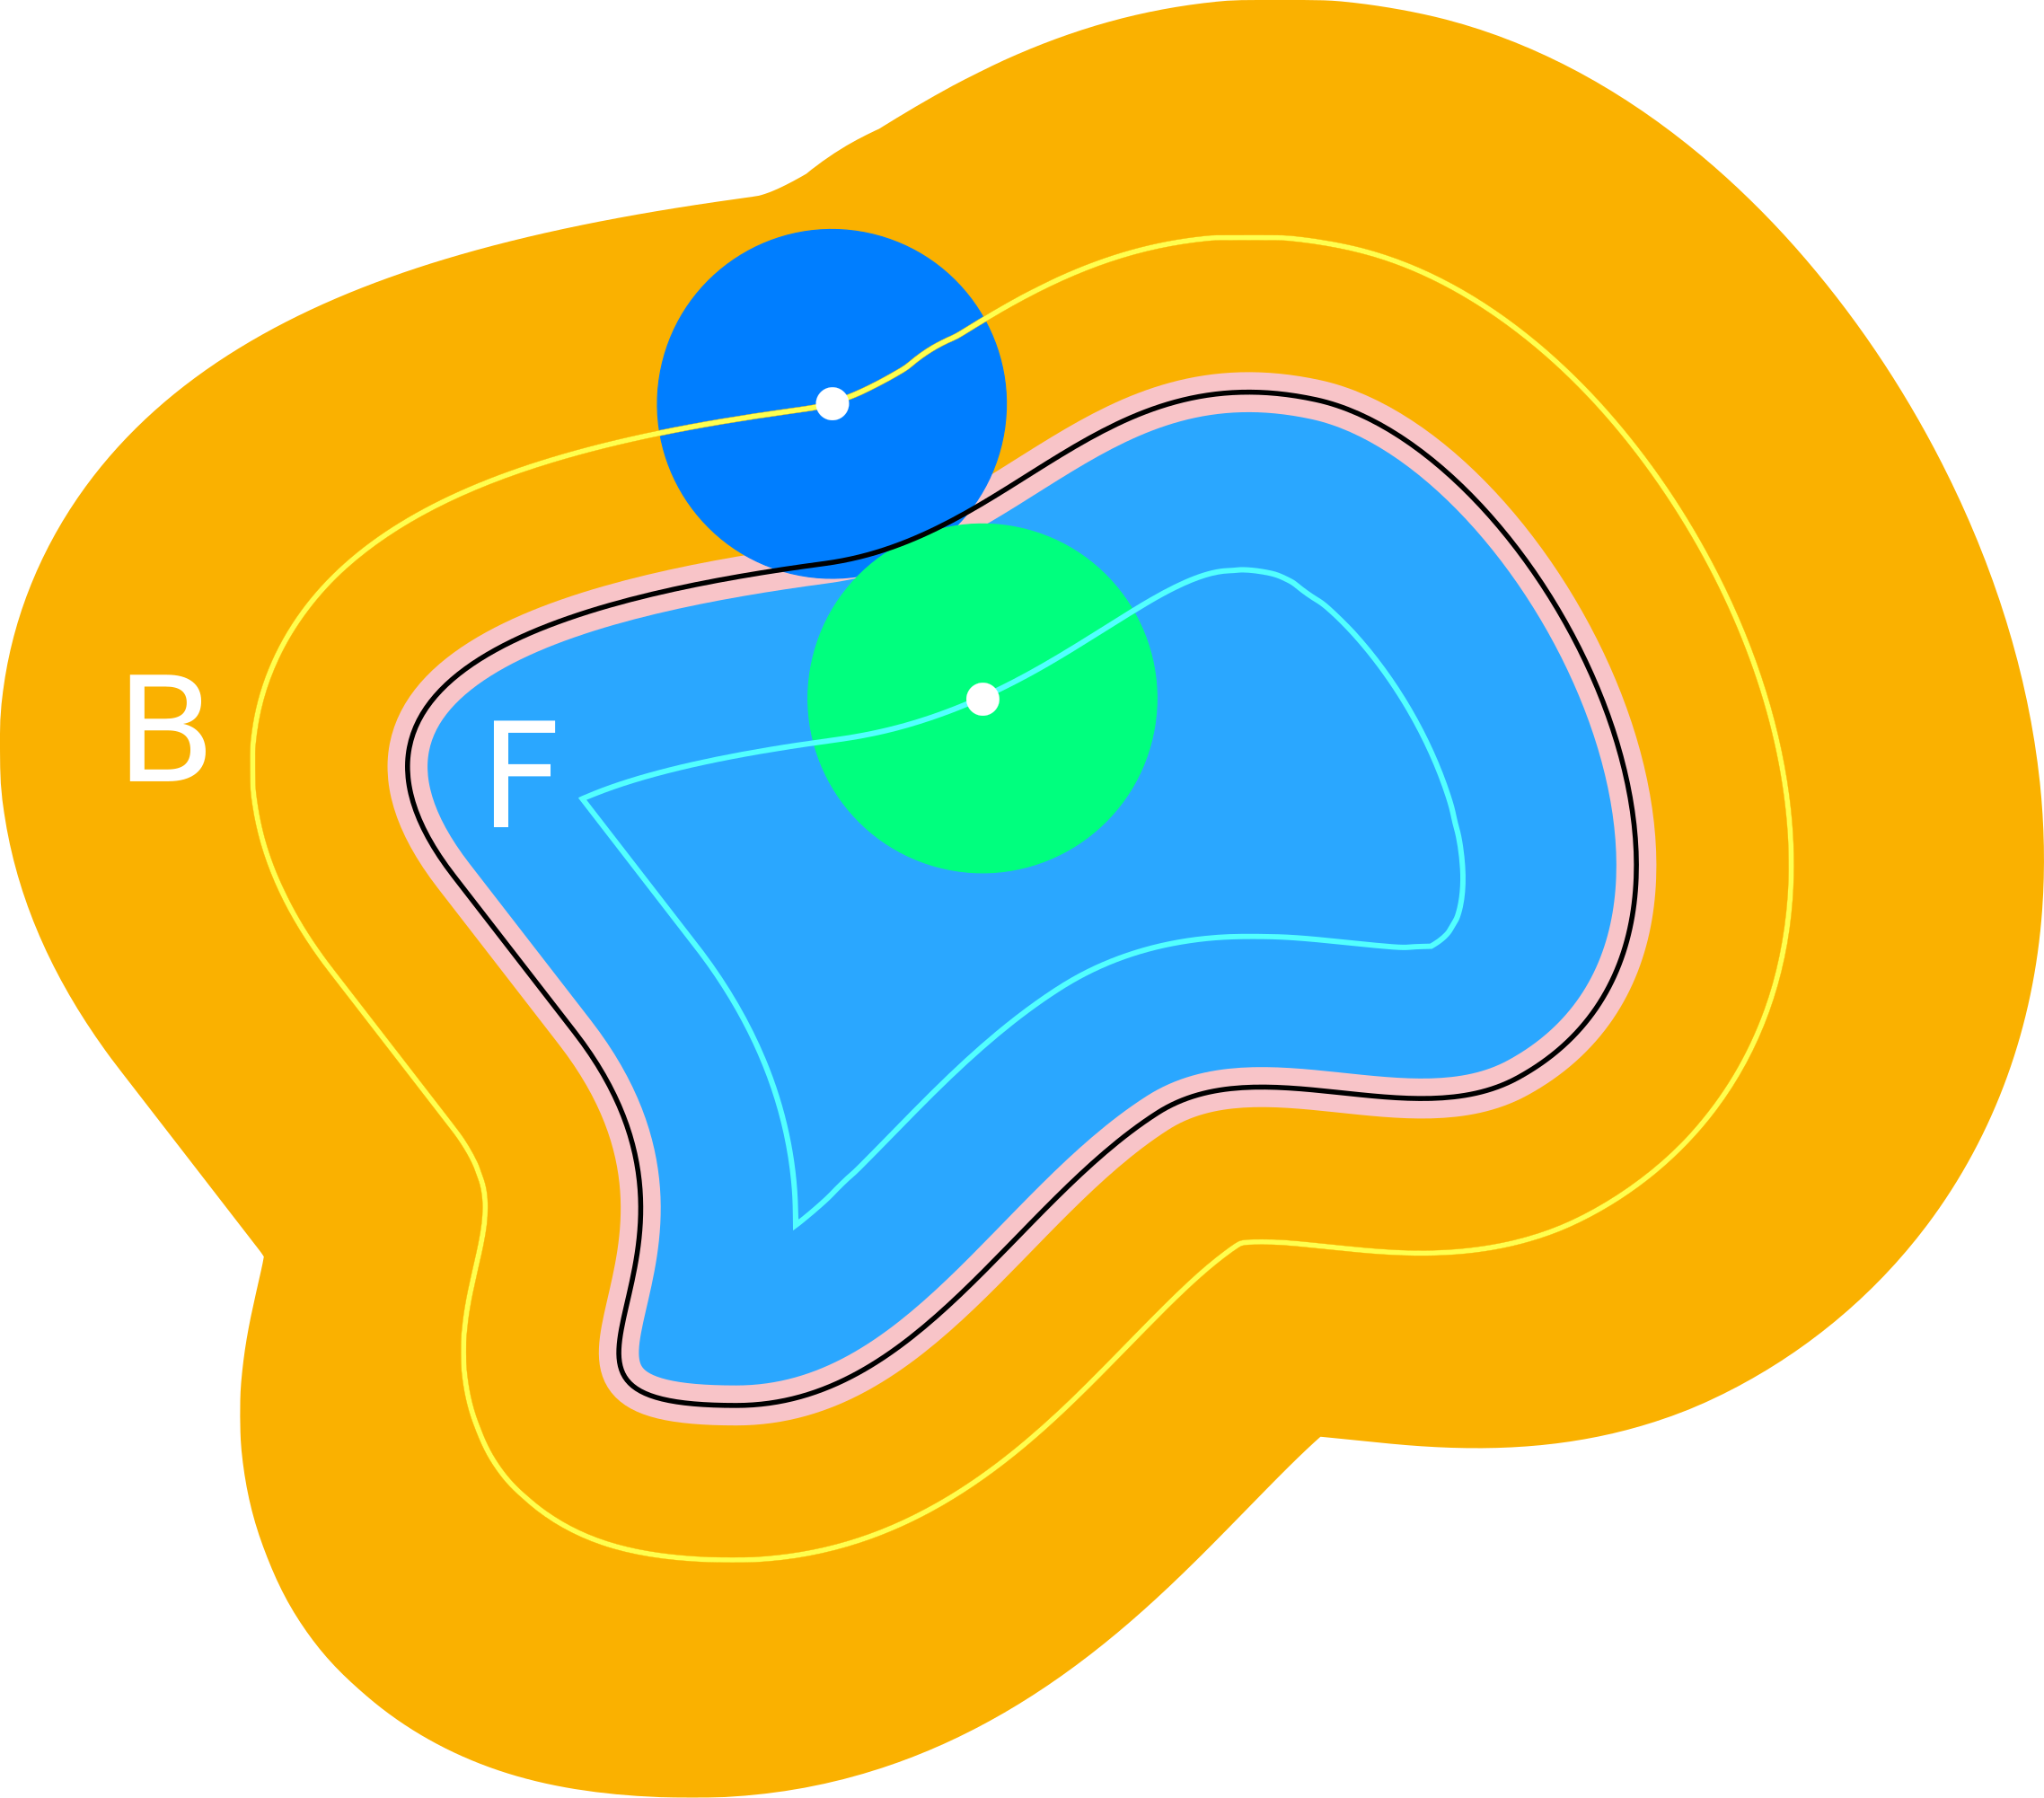
\includegraphics[scale=0.25]{figures/chapter5/max-energy/integral-2.png}
\caption{The estimation balls are evaluated along the inner and outer curves.}
\end{figure}


We evolve a curve evolution process in which at every step the following optimization process is solved

\begin{align}\label{eq:max-energy}
	\max_{x \in O}{E} &= \max_{x \in O} \sum_{p \in \mathcal{C}_{out}}{g_o} + \sum_{p \in \mathcal{C}_{inn}}{g_i}\\\nonumber 
	&=\sum_{p \in \mathcal{C}_{out}}{ \big( \pi R^2 - F_p - \sum_{x \in O_p}{x}\big)^2} + \sum_{p \in \mathcal{C}_{inn}}{ \big( F_p + \sum_{x \in O_p}{x}\big)^2}\\\nonumber
	&= \sum_{p \in \mathcal{C}_{out}}{ (1 - 2\pi R^2 + 2F_p) \sum_{x \in O_p}{x} + \sum_{ \substack{ x_j,x_k \in O_p \\ j < k}}{2x_jx_k}}\\\nonumber
	&+ \sum_{p \in \mathcal{C}_{inn}}{(2F_p + 1)\sum_{x \in O_p}{x} + \sum_{\substack{ x_j,x_k \in O_p \\ j < k}}{2x_jx_k}}	
\end{align}
